% !TEX program = xelatex
% ---------------------------------------------------------------------------
%  Solar Chromosphere Velocity (v2) — Method and Implementation Manual
%  Build:   latexmk -pdf -pdflatex="xelatex %O %S" manual.tex
%           (or simply:  latexmk -xelatex manual.tex)
% ---------------------------------------------------------------------------
\documentclass[11pt,a4paper]{article}

\usepackage[T1]{fontenc}
\usepackage{lmodern}
\usepackage{amsmath,amssymb,bm}
\usepackage{booktabs}
\usepackage{longtable}
\usepackage{graphicx}
\usepackage{geometry}
\usepackage{array}
\usepackage{tikz}
\usetikzlibrary{arrows.meta,positioning}
\usepackage{xcolor}
\usepackage[colorlinks=true,linkcolor=blue!55!black,citecolor=blue!55!black,
            urlcolor=blue!55!black]{hyperref}
\usepackage{enumitem}
\setlist{nosep,leftmargin=1.6em}

\geometry{margin=2.4cm}
\linespread{1.12}

\newcommand{\code}[1]{\texttt{\small #1}}
\newcommand{\vlos}{V_{\mathrm{LOS}}}
\newcommand{\Rsun}{R_{\odot}}
\newcommand{\Proj}{\mathcal{P}}
\newcommand{\Merid}{\mathcal{M}}

\title{\bfseries Solar Chromosphere Velocity (v2)\\[2mm]
       \large Method and Implementation Manual\\[1mm]
       \normalsize Program flow, streaming framework, spectral fitting and
       the velocity model}
\author{\code{solar-chromosphere-velocity} v2.1}
\date{\today}

\begin{document}
\maketitle

\begin{abstract}
\noindent
This manual documents the method and implementation of
\code{solar-chromosphere-velocity} v2.  The program takes CHASE/HIS level-1
spectral cubes, inverts the line-of-sight (LOS) velocity field, and decomposes
it into components with distinct physical meaning: differential rotation, a
limb shift, meridional circulation and a systemic translational velocity.  The
document covers the program flow and its timed stages, the streaming read plus
batched-FFT framework, the line-centre fit and the cross-correlation Doppler
inversion, the complete velocity model together with the physical meaning and
explicit expression of every term, parameter estimation and identifiability,
the output contract, and the measured speed-up over v1.0.1.  Every equation is
tied to the code that implements it, and example products for both H$\alpha$
and Fe\,\textsc{i} are included in Section~\ref{sec:examples}.
\end{abstract}

\tableofcontents
\vspace{4mm}

% ===========================================================================
\section{Introduction and scope}
% ===========================================================================

\subsection{Input}
CHASE (Xihe) HIS level-1 spectral cubes, typically of shape
$(\text{wavelength}, y, x) = (118, 2313, 2304)$ for H$\alpha$
(6562.82\,\AA, \code{SPECLINE='HA'}) or $(46, 2313, 2304)$ for Fe\,\textsc{i}
(6569.22\,\AA, \code{SPECLINE='FEI'}).  The cube is normally stored RICE\_1
tiled-compressed in \code{hdu[1]}, with the simultaneous 2-D line-core
intensity image in HDU~0.  Inputs that are already 2-D LOS velocity maps
(for example the \code{*\_Vdop.fits} products written by v1.0.1) are also
accepted.

\subsection{Output}
One multi-extension FITS file per observation time, containing ten 2-D layer
extensions plus a parameter table, together with an \code{index.csv}
observation log and optionally multi-panel PNG figures.  Outputs are
\textbf{never} written next to the inputs.

\subsection{Scope and limitations}
\begin{itemize}
  \item Physical assumptions: a single absorption line, an LOS velocity that is
        linear in the line-centre displacement, and a large-scale flow field
        described over a full-disk image by the nine-parameter analytic model
        of Section~\ref{sec:model}.
  \item The method returns a \emph{relative} LOS velocity.  The inversion
        template is the average profile of the disk-centre region, so any
        absolute (gravitational plus convective) line shift is already contained
        in the template.  The parameter $G$ is a systemic shift relative to that
        template and \textbf{must not be read as a gravitational redshift}.
  \item The method is not intended for local flows in strong active regions, nor
        for multi-component profiles (for example H$\alpha$ with pronounced
        wing emission).
\end{itemize}

% ===========================================================================
\section{Program flow}
\label{sec:flow}
% ===========================================================================

\subsection{Stages}
\code{process\_file()} in \code{processor.py} splits one file into the timed
stages listed in Table~\ref{tab:stages}; each stage records its wall time in
\code{ProcessResult.timings}.

\begin{figure}[htbp]
\centering
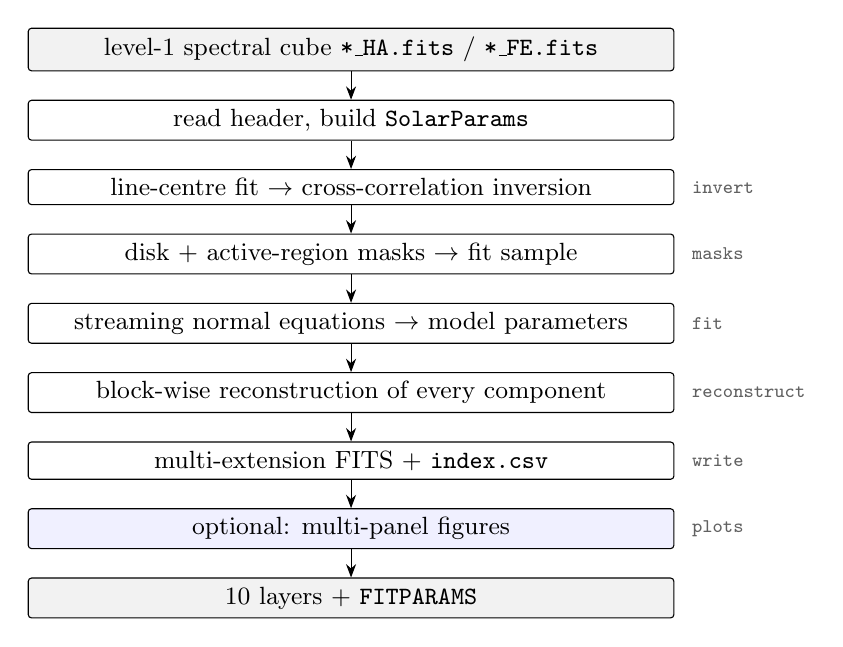
\begin{tikzpicture}[
  node distance=3.6mm,
  box/.style={draw, rounded corners=1.2pt, align=center, inner sep=3.2pt,
              font=\small, minimum width=82mm},
  io/.style={box, fill=black!5},
  key/.style={font=\scriptsize\ttfamily, text=black!62},
  >={Stealth[length=1.7mm]}
]
\node[io] (in)  {level-1 spectral cube \code{*\_HA.fits} / \code{*\_FE.fits}};
\node[box, below=of in]   (read) {read header, build \code{SolarParams}};
\node[box, below=of read] (inv)  {line-centre fit $\to$ cross-correlation inversion};
\node[box, below=of inv]  (msk)  {disk + active-region masks $\to$ fit sample};
\node[box, below=of msk]  (fit)  {streaming normal equations $\to$ model parameters};
\node[box, below=of fit]  (rec)  {block-wise reconstruction of every component};
\node[box, below=of rec]  (wrt)  {multi-extension FITS + \code{index.csv}};
\node[box, below=of wrt, fill=blue!6] (pl) {optional: multi-panel figures};
\node[io,  below=of pl]   (out)  {10 layers + \code{FITPARAMS}};

\draw[->] (in) -- (read);
\draw[->] (read) -- (inv);   \node[key,right=1mm of inv]  {invert};
\draw[->] (inv) -- (msk);    \node[key,right=1mm of msk]  {masks};
\draw[->] (msk) -- (fit);    \node[key,right=1mm of fit]  {fit};
\draw[->] (fit) -- (rec);    \node[key,right=1mm of rec]  {reconstruct};
\draw[->] (rec) -- (wrt);    \node[key,right=1mm of wrt]  {write};
\draw[->] (wrt) -- (pl);     \node[key,right=1mm of pl]   {plots};
\draw[->] (pl) -- (out);
\end{tikzpicture}
\caption{Per-file processing flow.  The small labels on the right are the keys
written into \code{timings}.}
\label{fig:flow}
\end{figure}

\noindent
The input type is decided before the flow starts, by
\code{data\_loader.detect\_data\_type()}: a 3-D cube goes through the spectral
inversion, a 2-D velocity map goes straight to the model fit.  For 2-D input the
\code{BUNIT} is honoured (\code{m/s} is converted to \code{km/s}); a map whose
unit is neither a velocity nor recognisable is refused by default, so that an
intensity image cannot silently be fitted as if it were a velocity.

\begin{table}[htbp]
\centering
\small
\caption{Timed stages (\code{ProcessResult.timings}).}
\label{tab:stages}
\begin{tabular}{lll}
\toprule
key & content & main code \\
\midrule
\code{read+invert}  & read plus inversion & \code{processor.\_read\_input} \\
\code{invert}       & inversion only & \code{inversion.DopplerInverter.run} \\
\code{masks}        & disk and active-region masks & \code{masks.active\_region\_mask} \\
\code{fit}          & least-squares model fit & \code{models.fit\_model\_streaming} \\
\code{reconstruct}  & component and error surfaces & \code{processor.\_reconstruct\_blocks} \\
\code{write}        & FITS and log & \code{output.write\_multihdu} \\
\code{plots}        & multi-panel figures (optional) & \code{plotting} \\
\code{total}        & single file, total & --- \\
\bottomrule
\end{tabular}
\end{table}

\subsection{Batch mode and naming}
\code{process\_directory()} calls \code{process\_file()} for each input and
writes one row per input into \code{index.csv}, including failed inputs.  The
output path is determined by the \textbf{observation time in the header}:
\begin{center}
\code{<output\_dir>/<YYYYMMDD>/<YYYYMMDD>T<HHMMSS>\_<LINE>\_scv.fits}
\end{center}
The time is taken from \code{STR\_TIME}, falling back to \code{DATE-OBS}, then
to a time parsed from the file name or its modification time.  Which one was
used is recorded in the \code{source} column of \code{index.csv} and in the
\code{TIMEKEY} header card.  Different observation times therefore
\textbf{cannot overwrite each other}, independently of the file names.  If the
target name already exists and \code{overwrite\_existing} is off, the program
adds a suffix rather than overwriting silently.

% ===========================================================================
\section{Reading and the streaming strategy}
% ===========================================================================

A RICE\_1 tiled-compressed FITS cube is a \code{CompImageHDU} in astropy.
Touching \code{hdu.data} decompresses the entire cube into memory, whereas
\code{hdu.section[...]} decodes only the requested tiles.  v2 uses the latter
throughout and advances in strips of \code{spatial\_strip\_rows} rows
(default 32):
\begin{equation}
  \text{cube } (n_\lambda, n_y, n_x) \;\longrightarrow\;
  \underbrace{(n_\lambda^{\mathrm{win}},\, s,\, n_x)}_{\text{one strip}},
  \qquad s = \code{spatial\_strip\_rows}.
\end{equation}
The strip height is a measured compromise: on a $2313\times2304$ RICE cube,
32 rows gave both the smallest peak memory and the shortest inversion time
against 64, 128, 256 and 512 rows.  The strategy makes memory essentially
independent of the image area and proportional only to the strip area.

% ===========================================================================
\section{Solar geometry}
\label{sec:geometry}
% ===========================================================================

For every pixel, the offset from disk centre is first rotated by the instrument
roll angle $P_0$ (header \code{INST\_ROT}):
\begin{equation}
\begin{pmatrix} x_r \\ y_r \end{pmatrix}
=
\begin{pmatrix} \cos P_0 & -\sin P_0 \\ \sin P_0 & \cos P_0 \end{pmatrix}
\begin{pmatrix} x - x_c \\ y - y_c \end{pmatrix},
\qquad
r = \sqrt{x_r^2 + y_r^2},
\end{equation}
where $(x_c, y_c)$ is the disk-centre pixel and $\Rsun$ is the solar radius in
pixels (header \code{R\_SUN}).  Assuming an orthographic projection, set
$\sin\rho = r/\Rsun$ and $\rho = \arcsin(r/\Rsun)$; with the position angle
$\theta$ defined by $\cos\theta = y_r/r$ and $\sin\theta = -x_r/r$, the
heliographic coordinates follow from
\begin{align}
  \sin B &= \sin B_0 \cos\rho + \cos B_0 \sin\rho \cos\theta, \\
  \sin L &= -\,\frac{\sin\rho\,\sin\theta}{\cos B},
\end{align}
where $B$ is the heliographic latitude, $L$ the longitude, and $B_0$ the
disk-centre latitude (header \code{B0}).  At the disk centre $r=0$ the position
angle is undefined; the implementation uses the $r\to0$ limit
($\cos\theta=1$, $\sin\theta=0$).  The routine also returns
$\mu = \cos\rho$, the limb-darkening geometrical factor.

\medskip
\noindent\textbf{Code:} \code{geometry.solar\_coords()}, with the batch version
\code{geometry.coord\_arrays()}.  The whole pipeline uses the vectorised form;
it measured about $59\times$ faster than v1's per-pixel scalar loop.

% ===========================================================================
\section{Spectral line-centre fitting}
\label{sec:linecenter}
% ===========================================================================

The first inversion step is to establish which wavelength sample holds the line
centre.  The program takes the mean profile inside
\code{reference\_profile\_radius} pixels of disk centre (default 100) as the
reference profile $\bar I(j)$ and locates the centre on it.

\subsection{The wavelength solution as a hint}
If the header contains \code{CDELT3}, \code{CRVAL3} and \code{WAVE\_LEN} (or a
recognisable \code{SPECLINE}), the linear wavelength solution
\begin{equation}
  \lambda(i) = \mathrm{CRVAL3} + \bigl(i - (\mathrm{CRPIX3}-1)\bigr)\,\mathrm{CDELT3}
\end{equation}
can be inverted for the line-centre sample,
\begin{equation}
  i_\star = \frac{\lambda_0 - \mathrm{CRVAL3}}{\mathrm{CDELT3}} + (\mathrm{CRPIX3}-1),
  \label{eq:wcscenter}
\end{equation}
with $\lambda_0$ the rest wavelength from \code{WAVE\_LEN} or looked up from
\code{SPECLINE}.  \textbf{This is only a hint}: in the level-1 data examined
here the wavelength solution and the data themselves disagree by about
1.4 pixels ($\sim$3\,km\,s$^{-1}$), so the centre must be measured from the data.

\subsection{Gaussian refinement}
Around the local minimum of $\bar I$ the program fits
\begin{equation}
  I(i) = I_c + A \exp\!\left[-\frac{(i-i_0)^2}{2\sigma^2}\right]
\end{equation}
by least squares, giving the continuous line centre $i_0$
(\code{LineCenter.index} is the rounded integer, \code{continuous} is $i_0$).
With \code{--legacy} the v1 threshold method
(\code{linecenter.\_legacy\_center}) is used instead, to reproduce v1.

% ===========================================================================
\section{Doppler velocity inversion}
\label{sec:inversion}
% ===========================================================================

\subsection{Correlation window}
With line centre $i_0$ and half-width $w = \code{correlation\_half\_width}$
(default 10), the window is $[i_0-w,\; i_0+w]$ of length $L = 2w+1$.  The
reference signal is the average profile inside that window,
\begin{equation}
  T(j) = \bar I(i_0-w+j), \qquad j = 0,\dots,L-1 .
\end{equation}
When continuum subtraction is enabled (\code{continuum\_subtraction}, on by
default outside legacy mode) the mean of each window is removed from both the
reference and the measured signal:
\begin{equation}
  \tilde T(j) = T(j) - \bar T, \qquad
  \tilde S_p(j) = S_p(j) - \bar S_p .
\end{equation}
Removing the window mean suppresses the bias that a continuum slope would
otherwise introduce into the peak position.

\subsection{Cross-correlation and sub-pixel refinement}
For each spatial pixel $p$ with observed window $S_p(j)$, the circular
cross-correlation is
\begin{equation}
  C_p(k) = \sum_{j=0}^{L-1} \tilde S_p(j)\, \tilde T(j-k),
  \label{eq:cc}
\end{equation}
evaluated for an entire strip at once through the FFT,
\begin{equation}
  C_p = \mathrm{IFFT}\!\left[\mathrm{FFT}(\tilde S_p)\cdot
        \overline{\mathrm{FFT}(\tilde T)}\right],
\end{equation}
followed by \code{fftshift} to place zero lag at $k = \lfloor L/2 \rfloor$.

With the peak at $k^\star = \arg\max_k C_p(k)$, a three-point parabola gives the
sub-pixel refinement
\begin{equation}
  x = \frac{C_p(k^\star-1) - C_p(k^\star+1)}
           {2\bigl[C_p(k^\star-1) - 2C_p(k^\star) + C_p(k^\star+1)\bigr]},
  \label{eq:parab}
\end{equation}
so the displacement relative to the window centre, in wavelength samples, is
\begin{equation}
  \delta_p = \bigl(k^\star + x\bigr) - \Bigl\lfloor \frac{L}{2} \Bigr\rfloor .
  \label{eq:disp}
\end{equation}
If $k^\star$ sits on a window edge the parabolic term is dropped and the integer
peak is used, which avoids extrapolating beyond the window.  Outside legacy mode
$x$ is clipped to $[-0.5,\,0.5]$ (\code{limit\_subpixel\_shift}).

\subsection{Velocity calibration}
From the dispersion $\mathrm{CDELT3}$ (\AA/pixel) and the rest wavelength
$\lambda_0$, one sample corresponds to
\begin{equation}
  \kappa \;=\; \frac{c\,\mathrm{CDELT3}}{\lambda_0},
  \qquad c = 299792.458\ \mathrm{km\,s^{-1}},
  \label{eq:scale}
\end{equation}
hence the LOS velocity
\begin{equation}
  \boxed{\;\vlos(p) \;=\; \delta_p \cdot \kappa\;}
  \label{eq:vlos}
\end{equation}
For H$\alpha$ ($\mathrm{CDELT3}=0.04844$\,\AA, $\lambda_0=6562.82$\,\AA) this
gives $\kappa \approx 2.2139$\,km\,s$^{-1}$/pixel.  With \code{--legacy} the
v1 hard-coded constant $\kappa_{\rm v1} = 1.1068\times2 = 2.2136$
km\,s$^{-1}$/pixel is used instead.  Off-limb pixels ($r>\Rsun$) are set to 0
following v1 semantics, and pixels beyond
$\code{disk\_mask\_radius}\cdot\Rsun$ are set to \code{NaN} so that they take no
part in the fit.  The sign convention is \textbf{redshift (receding) positive},
recorded in the \code{UNITSYS} card.

% ===========================================================================
\section{The velocity model}
\label{sec:model}
% ===========================================================================

\subsection{The model equation}
Write $B$ for heliographic latitude (with $s_B \equiv \sin B$), $L$ for
longitude and $\rho$ for the heliocentric angle, and define the two LOS
projection factors
\begin{align}
  \Proj  &= \cos B \,\sin L \,\cos B_0, \label{eq:proj-rot}\\
  \Merid &= \cos L \,\sin B \,\cos B_0 \;-\; \cos B \,\sin B_0 . \label{eq:proj-mer}
\end{align}
$\Proj$ is the LOS projection of the rotation velocity (directed along
longitude) and $\Merid$ is the LOS projection of the meridional circulation
after expanding it on the two unit vectors $(\hat B, \hat L)$.  The model LOS
velocity is then
\begin{equation}
\boxed{
\begin{aligned}
V_{\mathrm{model}}(B,L,\rho) =\;&
  s\Bigl(A + B s_B^{2} + C s_B^{4} + D \sin^{10}\!\rho\Bigr)\Proj
  \quad\text{(differential rotation)}\\
 &+\; e\,\bigl(1-\cos\rho\bigr)^{N} \qquad\qquad\ \ \text{(limb shift)}\\
 &+\; \bigl(\mathrm{MC1}\,s_B + \mathrm{MC2}\,\sin 2B\bigr)\Merid
  \qquad\ \text{(meridional circulation)}\\
 &+\; G \qquad\qquad\qquad\qquad\qquad\quad\ \ \text{(systemic translation)}
\end{aligned}}
\label{eq:model}
\end{equation}
where $s = \Rsun = 6.957\times10^{5}$\,km when the rotation parameters are given
as angular rates (\code{rotation\_amplitude='rad\_per\_s'}), and $s = 1$
otherwise (velocity amplitudes in km/s).

\subsection{Physical meaning of each term}
Table~\ref{tab:terms} lists the nine parameters, what each denotes and its
complete expression.  The parameter order
\code{TERM\_ORDER}${}=(A,B,C,D,G,e,N,\mathrm{MC1},\mathrm{MC2})$ is the same as
in v1, so historical parameter files can be compared directly.

\begin{table}[htbp]
\centering
\small
\caption{Model parameters, physical meaning and expression.  All amplitudes are
in km/s; $N$ is dimensionless.}
\label{tab:terms}
\begin{tabular}{@{}lll@{}}
\toprule
parameter & physical meaning & expression \\
\midrule
$A$ & equatorial rotation amplitude (constant term of the $\Omega$ expansion)
    & $s\,A\,\Proj$ \\
$B$ & rotation, $\sin^2 B$ term (differential rotation)
    & $s\,B\,s_B^{2}\,\Proj$ \\
$C$ & rotation, $\sin^4 B$ term
    & $s\,C\,s_B^{4}\,\Proj$ \\
$D$ & rotation, $\sin^{10}\!\rho$ limb term
    & $s\,D\,\sin^{10}\!\rho\,\Proj$ \\
$e$ & limb-shift amplitude (\code{limb\_amplitude\_positive} constrains $e\ge0$)
    & $e\,(1-\cos\rho)^{N}$ \\
$N$ & power-law exponent of the limb shift (chosen on a grid)
    & $(1-\cos\rho)^{N}$ \\
$\mathrm{MC1}$ & meridional circulation, $\sin B$ component
    & $\mathrm{MC1}\,s_B\,\Merid$ \\
$\mathrm{MC2}$ & meridional circulation, $\sin 2B$ component
    & $\mathrm{MC2}\,\sin 2B\,\Merid$ \\
$G$ & systemic translational velocity (global zero point of the model)
    & $G$ \\
\bottomrule
\end{tabular}
\end{table}

\noindent
\textbf{On $G$.}  The inversion template is the disk-centre average profile, so
$G$ absorbs three things at once: a genuine systemic velocity, the offset
between that template and the rest wavelength, and the absolute wavelength zero
point of the instrument.  It is mathematically degenerate with the choice of
template, with the zero-point correction \code{zero\_point\_km\_s}, and with the
mean removed by continuum subtraction.  It must therefore be read as a
\emph{systemic zero-point reading only, never as a gravitational redshift}.  For
reference the nominal gravitational redshift is
$GM/(\Rsun c) \approx 0.636$\,km\,s$^{-1}$, whereas measured values of $|G|$ are
around $0.014$--$0.20$\,km\,s$^{-1}$ depending on the line and the event; the two
are not of the same order.

\subsection{Degenerate cases}
When a line carries no measurable limb shift over the full disk (as is the case
for disk-averaged H$\alpha$), the linear least-squares solution may return
$e<0$.  If \code{limb\_amplitude\_positive} is set, the program then pins $e$ to
the boundary $e=0$ (an active-set step), so $V_{\rm LIMB}\equiv0$ and $N$ has no
influence on the model whatsoever: neither parameter is identifiable.  Both are
flagged and given \code{NaN} errors (Section~\ref{sec:ident}).  For the Fe\,\textsc{i}
data examined here, $e\approx0.19$\,km\,s$^{-1}$ and is significantly positive,
so $V_{\rm LIMB}$ shows a genuine limb-brightening ring
(Figure~\ref{fig:fe-components}).

\subsection{Layers derived from the model}
\code{models.VelocityModel.components()} produces the layers in
Table~\ref{tab:layers}.  \code{V\_LARGE} is the sum of the four components (the
model surface) and \code{V\_RESID} is the observation minus that surface, with
the quiet-Sun mean (header \code{QUIETMN}) removed as well.

\begin{table}[htbp]
\centering
\small
\caption{Definition of the output layers (\code{output.LAYERS}).}
\label{tab:layers}
\begin{tabular}{@{}lll@{}}
\toprule
\code{EXTNAME} & physical meaning & expression \\
\midrule
\code{VLOS\_OBS}   & observed LOS velocity & $\delta_p\kappa$, Eq.~\eqref{eq:vlos} \\
\code{VLOS\_CORR}  & LOS velocity after the zero-point correction & $\vlos - \mathrm{ZEROPT}$ \\
\code{V\_DIFFROT}  & differential-rotation component & $s(A+B s_B^2+C s_B^4+D\sin^{10}\!\rho)\Proj$ \\
\code{V\_LIMB}     & limb-shift component & $e(1-\cos\rho)^N$ \\
\code{V\_MERID}    & meridional circulation, LOS projected & $(\mathrm{MC1}s_B+\mathrm{MC2}\sin2B)\Merid$ \\
\code{V\_OFFSET}   & systemic translation & $G$ \\
\code{V\_LARGE}    & total large-scale flow surface & sum of the four above \\
\code{V\_RESID}    & residual LOS velocity & $\code{VLOS\_CORR}-\code{V\_LARGE}-\code{QUIETMN}$ \\
\code{V\_MODEL\_ERR} & $1\sigma$ of the model surface & $\sqrt{\bm{x}^\top\Sigma\bm{x}}$ \\
\code{MASK\_ACTIVE} & active-region mask & $0$ quiet, $1$ active \\
\bottomrule
\end{tabular}
\end{table}

% ===========================================================================
\section{Parameter estimation, uncertainty and identifiability}
\label{sec:estimation}
% ===========================================================================

\subsection{Linear least squares and streaming normal equations}
Except for $N$, the model is linear in every parameter: for a given $N$ the
eight columns of the design matrix $\bm{X}$ are
$[\Proj,\ s_B^2\Proj,\ s_B^4\Proj,\ \sin^{10}\!\rho\,\Proj,\ (1-\cos\rho)^N,\
s_B\Merid,\ \sin2B\,\Merid,\ 1]$,
with parameter vector $\bm\beta = (A,B,C,D,e,\mathrm{MC1},\mathrm{MC2},G)^\top$.
Minimising
\begin{equation}
  \chi^2(\bm\beta) = \sum_{p}\bigl(\vlos^{(p)} - \bm{x}_p^\top\bm\beta\bigr)^2
\end{equation}
gives the normal equations $\bm{X}^\top\bm{X}\,\bm\beta = \bm{X}^\top\bm{y}$.
The program never forms the full design matrix; it accumulates strip by strip,
\begin{equation}
  \bm{X}^\top\bm{X} \mathrel{+}= \bm{X}_b^\top\bm{X}_b,\qquad
  \bm{X}^\top\bm{y} \mathrel{+}= \bm{X}_b^\top\bm{y}_b,\qquad
  y^\top y \mathrel{+}= \bm{y}_b^\top\bm{y}_b ,
\end{equation}
so memory is independent of the pixel count (a $9\times9$ matrix), and solves
the small system by Cholesky factorisation.

\subsection{Scanning $N$}
$N$ enters as a power-law exponent and cannot be solved linearly, so the program
solves the same normal equations for each value in
\code{limb\_exponent\_scan} (default $\{1,1.25,1.5,2,2.5,3,4,5\}$) and takes the
value with the smallest residual sum of squares.  All grid points share the
accumulators, so the extra cost is essentially zero.  The resulting $N$-RSS
curve is written into the parameter-table header (\code{NSCAN},
\code{NSCAN02}, \dots).

\subsection{The $e\ge0$ active-set step}
If the unconstrained solution gives $e<0$, the constrained optimum lies on the
boundary $e=0$: the program \textbf{drops the column for $e$} and re-solves.
This necessarily raises the residual sum of squares --- that is the price of the
constraint, not a reason to reject it.

\subsection{Uncertainty}
The covariance is $\Sigma = \hat\sigma^2 (\bm{X}^\top\bm{X})^{-1}$ with
$\hat\sigma^2 = \mathrm{RSS}/(n-p)$.  For a dropped column the corresponding row
and column of the covariance are zero.  The per-pixel model uncertainty written
to \code{V\_MODEL\_ERR} is
\begin{equation}
  \sigma_{\rm model}(\bm{x}) = \sqrt{\bm{x}^\top \Sigma\, \bm{x}} .
\end{equation}

\subsection{Identifiability and flags}
\label{sec:ident}
Reporting a numerical error for a parameter that is not identifiable would read
as a very precise measurement.  For the following cases the program therefore
sets the error to \code{NaN}, writes a \code{FLAG} in \code{FITPARAMS}, writes
\textbf{no} \code{ERR\_*} card for that parameter, and summarises them in the
\code{FITFLAG} card of \code{PRIMARY}:
\begin{itemize}
  \item \code{PINNED\_AT\_ZERO}: $e$ is constrained to $e=0$ (active-set step);
  \item \code{DEGENERATE\_WITH\_E}: with $e$ pinned, $N$ has no effect on the model;
  \item \code{FLAT\_SCAN}: the $N$ scan changes the RSS by a negligible amount;
  \item \code{SCAN\_GRID}: $N$ is chosen from a discrete grid and never has a
        covariance-based uncertainty.
\end{itemize}
Note that the covariance matrix itself is \textbf{not} set to \code{NaN}: only
the reported $1\sigma$ is.  Blanking the covariance would turn the entire
\code{V\_MODEL\_ERR} layer into \code{NaN}, because it is computed from
$\sqrt{\bm{x}^\top\Sigma\bm{x}}$.

% ===========================================================================
\section{Streaming and parallel framework}
\label{sec:parallel}
% ===========================================================================

The performance of v2 comes from three layers, in decreasing order of
contribution:

\begin{enumerate}
  \item \textbf{Vectorised solar geometry.}  $(B,L,\rho)$ is computed for every
        pixel of a strip in one operation, replacing v1's per-pixel Python loop
        ($\sim59\times$).
  \item \textbf{Batched-FFT cross-correlation.}  Eq.~\eqref{eq:cc} is evaluated
        for all pixels of a strip simultaneously: a single FFT along the
        wavelength axis of an array of shape $(L,\; s\cdot n_x)$
        ($\sim38\times$; $24.4$\,\textmu s $\to$ $0.65$\,\textmu s per pixel on
        synthetic data).
  \item \textbf{Streaming normal equations.}  The fit accumulates an
        $8\times8$ matrix strip by strip, so its memory does not grow with the
        number of pixels; the reconstruction is block-wise too, and only the ten
        output layers remain resident.
\end{enumerate}

\noindent
The configuration keys \code{parallel\_processing} and
\code{parallel\_processes} are \textbf{reserved}: single-file processing is
already fast (Section~\ref{sec:speed}), and parallelising across \emph{files}
with the scheduler is more efficient.  The in-process path is deliberately
single-threaded so that results are reproducible.

\paragraph{Complexity.}
With $P$ pixels, window length $L = 2w+1$ and strip height $s$: the inversion is
$\mathcal{O}(P L\log L)$, the fit is $\mathcal{O}(P\cdot 8^2)$, and the peak
memory is $\mathcal{O}(s\,n_x\,L + 10\,n_y n_x)$ --- the first term from the
strip, the second from the ten float32 output layers.

% ===========================================================================
\section{Output structure}
\label{sec:output}
% ===========================================================================

One observation time produces one FITS file with a fixed extension order:
\begin{center}
\code{PRIMARY}, \code{VLOS\_OBS}, \code{VLOS\_CORR}, \code{V\_DIFFROT},
\code{V\_LIMB}, \code{V\_MERID}, \code{V\_OFFSET}, \code{V\_LARGE},
\code{V\_RESID}, \code{V\_MODEL\_ERR}, \code{MASK\_ACTIVE}, \code{FITPARAMS}
\end{center}

\code{PRIMARY} carries the observation metadata (time, source file, disk
geometry, \code{CALSPEC}, \code{INVMETH}, \code{UNITSYS}, goodness of fit and
\code{FITFLAG}) and is guaranteed to contain \textbf{no duplicate keywords}.
Each velocity layer carries \code{BUNIT='km/s'}, \code{QUANTITY},
\code{FORMULA}, \code{PARAMS} and \code{MODELVER}.  \code{FITPARAMS} is a
nine-row binary table with columns \code{NAME, VALUE, ERROR, UNIT, COMPONENT,
FORMULA, DESCRIPTION, FLAG}.  \code{index.csv} has one row per input per run,
with the observation time, the source of that time, the output file name, the
model version, the number of fit points, the RMS, and the nine parameter values.

% ===========================================================================
\section{Differences from v1.0.1 and the measured speed-up}
\label{sec:speed}
% ===========================================================================

\begin{table}[htbp]
\centering
\small
\caption{Main physical and numerical differences.}
\begin{tabular}{@{}p{0.30\textwidth}p{0.62\textwidth}@{}}
\toprule
aspect & v2 relative to v1.0.1 \\
\midrule
velocity calibration & computed from the header \code{CDELT3}/\code{WAVE\_LEN}
                       (Eq.~\eqref{eq:scale}) instead of hard-coded $1.1068\times2$ \\
line centre & Gaussian fit with the wavelength solution as a hint; v1 used a threshold method \\
rotation projection & includes the $\cos B_0$ factor; v1 omitted it \\
meridional circulation & LOS projected via $\Merid$ (Eq.~\eqref{eq:proj-mer}); v1 did not project \\
continuum & correlation windows are mean-subtracted; v1 did not subtract \\
sub-pixel & the parabolic term is clipped to $\pm0.5$ pixel; v1 did not clip \\
reading & strip-wise \code{hdu.section} only; v1 decompressed the whole cube \\
fitting & streaming normal equations; v1 used per-pixel \code{curve\_fit} \\
output & one multi-extension FITS per observation time; v1 wrote single-layer files next to the inputs \\
\bottomrule
\end{tabular}
\end{table}

\begin{table}[htbp]
\centering
\small
\caption{Measured on BlueWhale (2026-04-24 H$\alpha$, $2313\times2304\times118$,
64-core \code{mpi} queue, conda environment with python 3.11, astropy 8.0.1,
numpy 2.4.6), single process.}
\label{tab:speed}
\begin{tabular}{@{}lrr@{}}
\toprule
implementation & wall time (s) & peak memory (GB) \\
\midrule
v1.0.1 (original)          & 169.17 & 4.266 \\
v2 \code{--legacy}         &   8.90 & 0.575 \\
v2 complete physics        &   9.59 & 0.583 \\
\midrule
speed-up (complete physics)& \multicolumn{2}{r}{$17.6\times$} \\
speed-up (\code{--legacy}) & \multicolumn{2}{r}{$19.0\times$} \\
memory ratio               & \multicolumn{2}{r}{$7.3\times$} \\
\bottomrule
\end{tabular}
\end{table}

\noindent
In the same run the v2 \code{VLOS\_OBS} differs from the v1 product by
$\max|\Delta| = 9.5\times10^{-7}$\,km\,s$^{-1}$ (rms $7.5\times10^{-8}$) and the
identifiable parameters by $\max|\Delta| = 4.4\times10^{-7}$: the two versions
describe the same curve, and the differences come from the physical corrections
listed above.

Note that \code{--visualize} is not free: the nine figures roughly double the
wall time and raise the peak from 0.58\,GB to about 1.5\,GB (three figures) or
3.0\,GB (nine figures).  A plotting failure never affects the FITS product.

% ===========================================================================
\section{Example products}
\label{sec:examples}
% ===========================================================================

The two figures below are real products of this version, drawn by the
\code{--visualize --plot-per-component} option, and are shown here as a
reference for what the layer set looks like in practice.  In both cases every
panel has its own symmetric colour scale, because the components differ by
orders of magnitude, and the axes are in arcseconds relative to disk centre
(derived from \code{CDELT1}/\code{CDELT2} and the disk centre).

\begin{figure}[htbp]
\centering
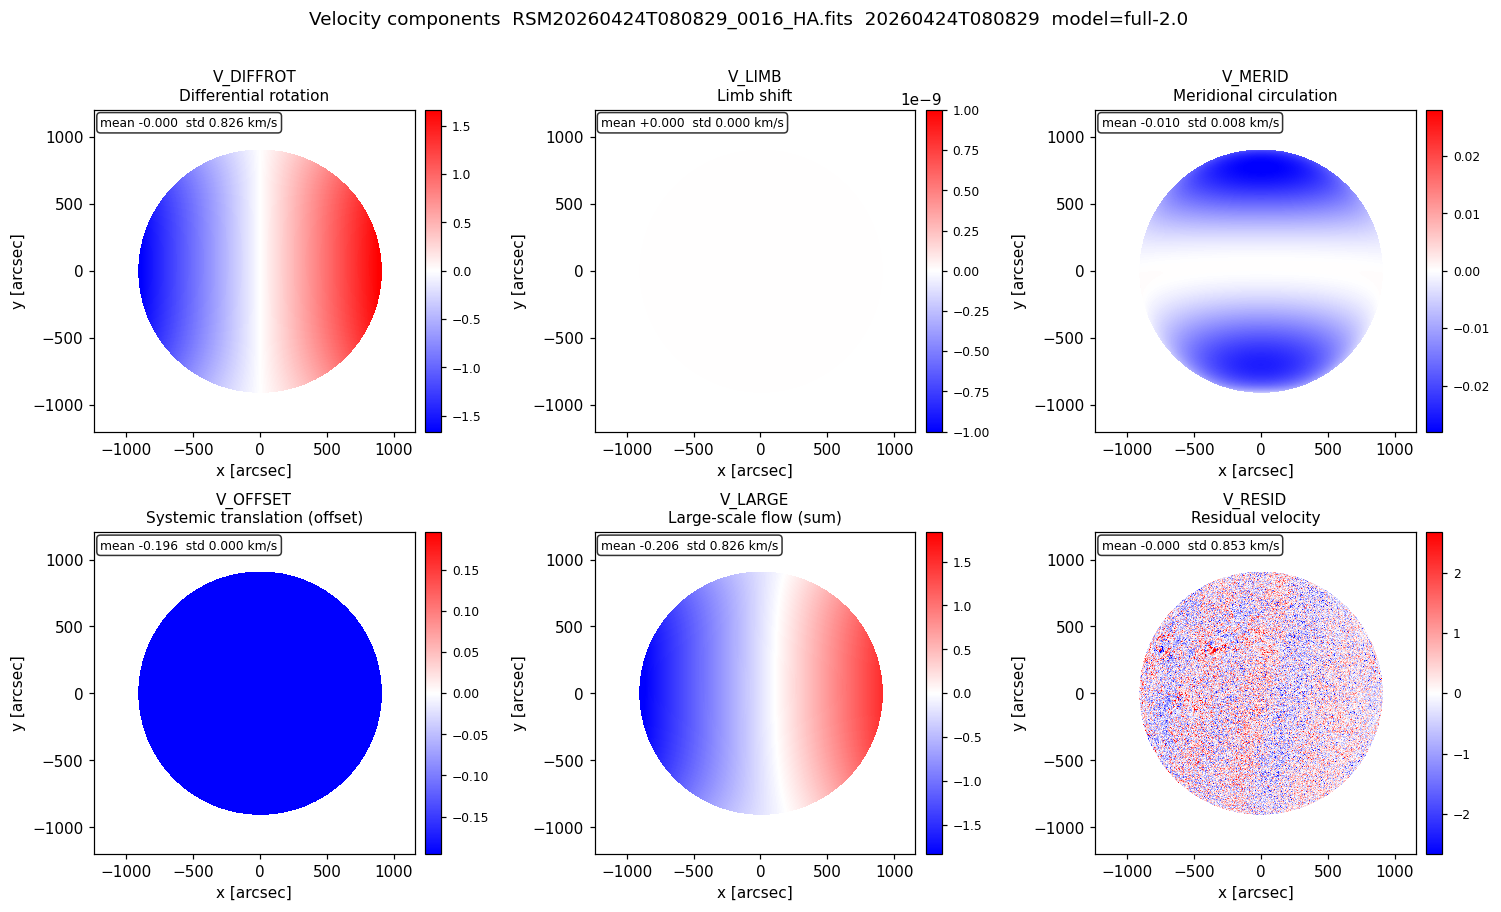
\includegraphics[width=\textwidth]{figs/ha_components.png}
\caption{H$\alpha$, 2026-04-24 08:08:29 UT
(\code{RSM20260424T080829\_0016\_HA.fits}).  The four model terms, their sum and
the residual.  \code{V\_DIFFROT} is the expected east--west antisymmetric
differential-rotation pattern ($\sigma=0.826$\,km\,s$^{-1}$),
\code{V\_MERID} is north--south antisymmetric ($\sigma=0.008$\,km\,s$^{-1}$),
\code{V\_OFFSET} is uniform at $-0.196$\,km\,s$^{-1}$ and
\code{V\_RESID} has $\sigma=0.853$\,km\,s$^{-1}$.  The \code{V\_LIMB} panel is
blank because for this line the fit pins $e$ to its lower bound $e=0$, so the
layer is identically zero (the colour bar spans $10^{-9}$\,km\,s$^{-1}$); the
parameter is flagged \code{PINNED\_AT\_ZERO} rather than reported as a
measurement.}
\label{fig:ha-components}
\end{figure}

\begin{figure}[htbp]
\centering
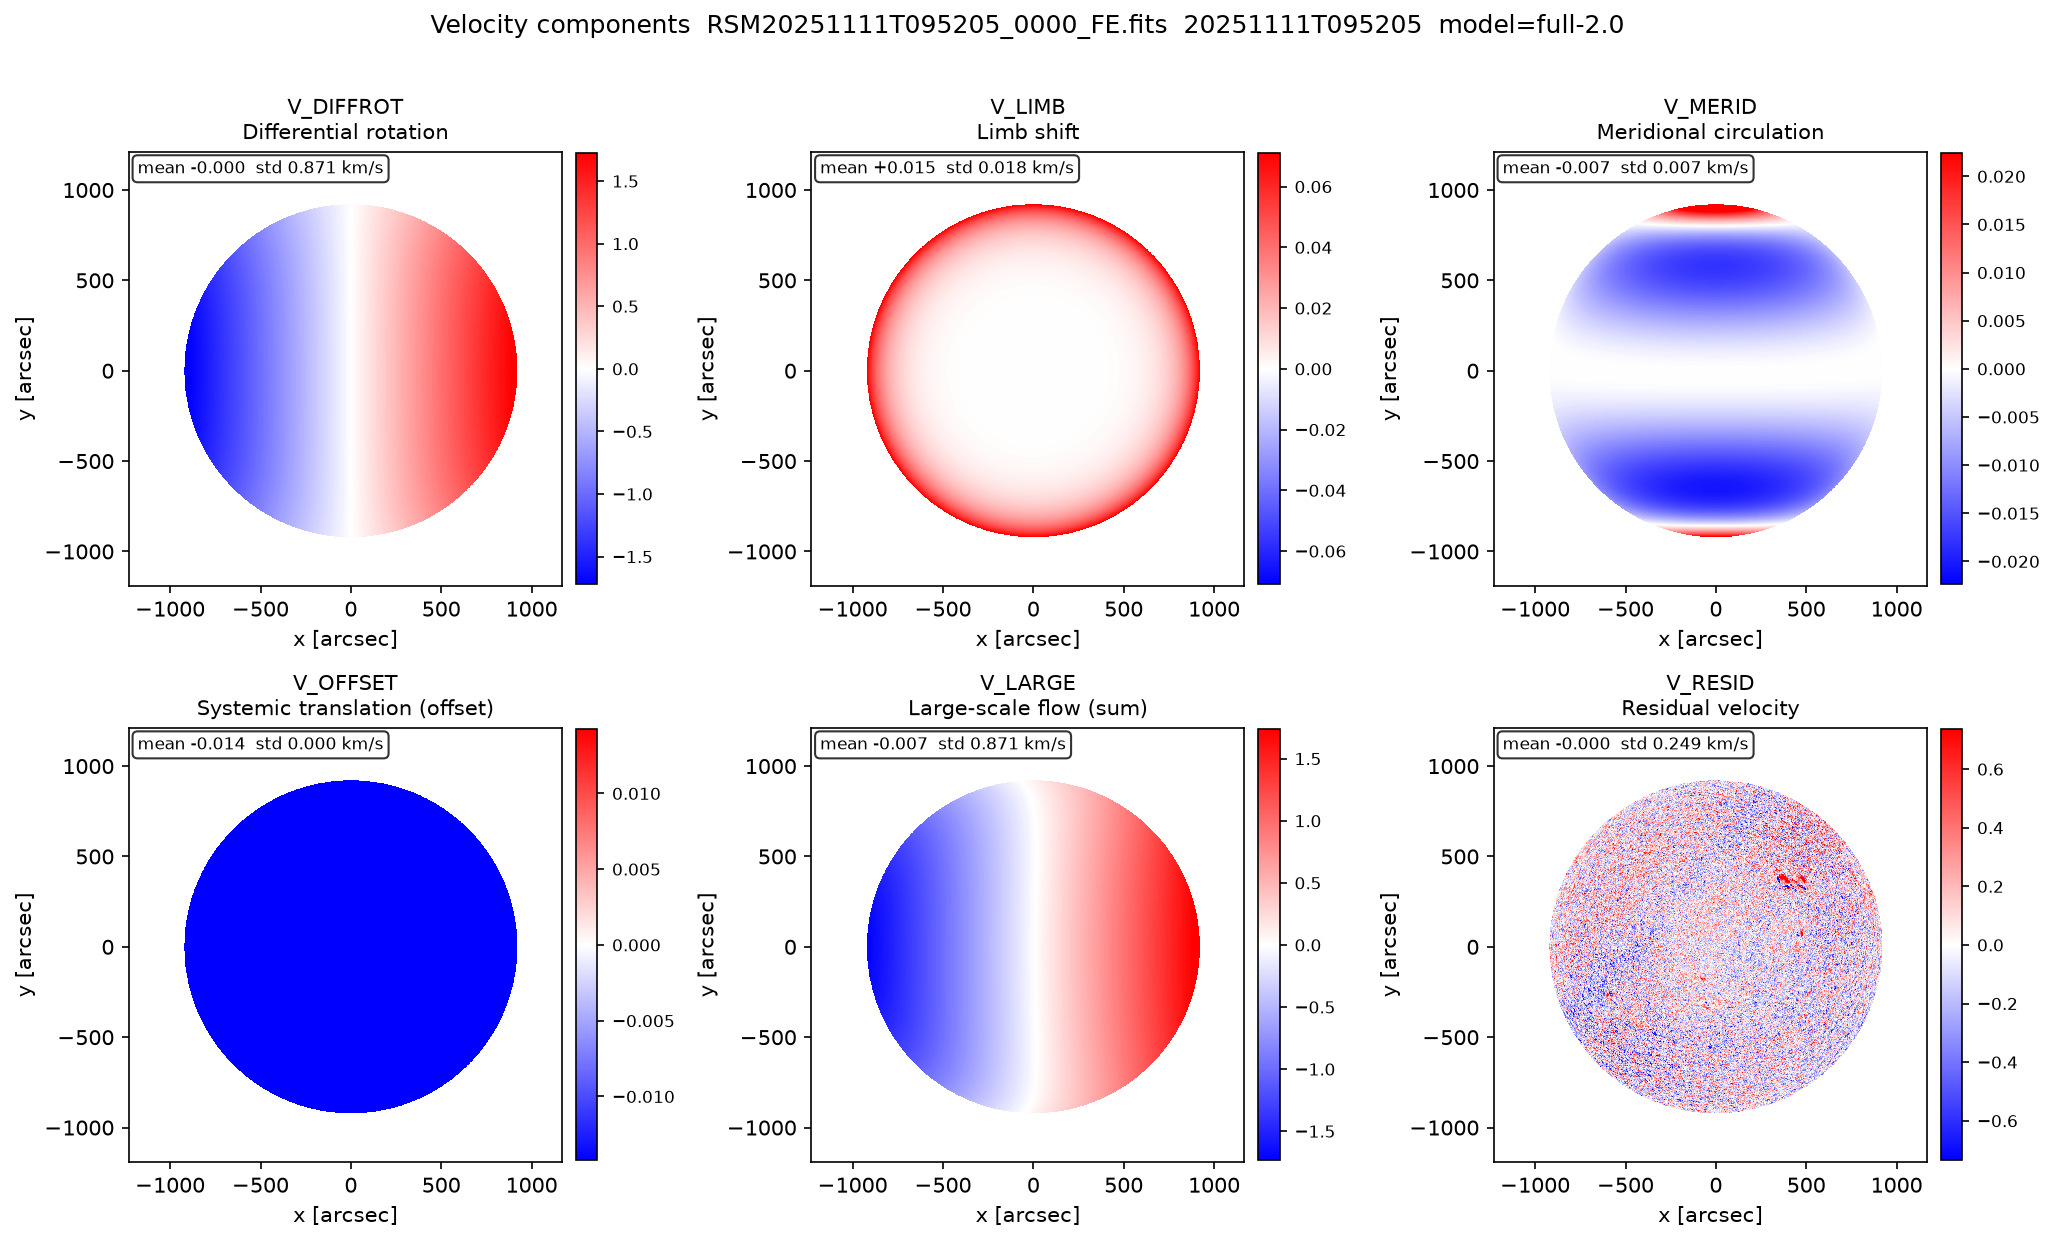
\includegraphics[width=\textwidth]{figs/fe_components.png}
\caption{Fe\,\textsc{i}, 2025-11-11 09:52:05 UT
(\code{RSM20251111T095205\_0000\_FE.fits}), from the same pipeline with no
change other than the input line: the dispersion gives
\code{CALSPEC}$\,=2.2108$\,km\,s$^{-1}$/pixel against $2.2139$ for H$\alpha$,
and the output is tagged \code{\_FEI}.  Here $e=0.186$\,km\,s$^{-1}$ is a
genuine positive fit, so \code{V\_LIMB} shows a real limb-brightening ring
rather than a blank panel, and the residual is three times smaller
($\sigma=0.249$\,km\,s$^{-1}$).  This pair of figures illustrates why
identifiability is reported explicitly: the same code flags \code{e} for
H$\alpha$ and does not flag it for Fe\,\textsc{i}, while $N$ is flagged
\code{SCAN\_GRID} in both cases.}
\label{fig:fe-components}
\end{figure}

% ===========================================================================
\appendix
\section{Symbols}
% ===========================================================================

\begin{longtable}{@{}ll@{}}
\toprule
symbol & meaning \\
\midrule
\endhead
$B$, $L$, $\rho$ & heliographic latitude, longitude, heliocentric angle \\
$B_0$            & disk-centre latitude (header \code{B0}) \\
$\mu=\cos\rho$   & limb-darkening geometrical factor \\
$\Rsun$          & solar radius: pixels via header \code{R\_SUN}; physically
                   $6.957\times10^5$\,km \\
$\delta_p$       & sub-pixel cross-correlation displacement of pixel $p$
                   (Eq.~\eqref{eq:disp}) \\
$\kappa$         & velocity calibration, km/s per pixel (Eq.~\eqref{eq:scale}) \\
$\Proj$, $\Merid$ & LOS projection factors of rotation and meridional
                   circulation (Eqs.~\eqref{eq:proj-rot}, \eqref{eq:proj-mer}) \\
$\bm{X},\bm\beta$ & design matrix and parameter vector \\
$w$              & correlation window half-width
                   (\code{correlation\_half\_width}) \\
$s$              & strip height (\code{spatial\_strip\_rows}) \\
\bottomrule
\end{longtable}

\section{Key configuration options (v2.1 names)}
% ===========================================================================

\begin{longtable}{@{}lll@{}}
\toprule
option & default & meaning \\
\midrule
\endhead
\code{limb\_exponent}             & \code{None} & fix the power-law exponent $N$; default is to scan \\
\code{limb\_exponent\_scan}       & $1\ldots5$  & grid of $N$ values \\
\code{limb\_amplitude\_positive}  & \code{True} & constrain $e\ge0$ \\
\code{correlation\_half\_width}   & 10 & correlation window half-width $w$ \\
\code{reference\_profile\_radius} & 100 & radius of the reference-profile average (pixels) \\
\code{continuum\_subtraction}     & on outside legacy & subtract the window mean \\
\code{limit\_subpixel\_shift}     & on outside legacy & clip the sub-pixel term to $\pm0.5$ \\
\code{min\_spectral\_samples}     & 90 & minimum samples for the legacy line-centre method \\
\code{disk\_mask\_radius}         & 0.95 & mask radius in units of $\Rsun$ \\
\code{active\_region\_sigma\_threshold} & 3.0 & active-region threshold in $\sigma$ \\
\code{active\_region\_robust\_sigma}    & on outside legacy & use a robust (MAD) $\sigma$ \\
\code{min\_active\_region\_area}  & 100 & minimum area of a detected region (pixels) \\
\code{active\_region\_grow\_steps}   & 3 & dilation steps for active regions \\
\code{active\_region\_shrink\_steps} & 1 & erosion steps for active regions \\
\code{spatial\_strip\_rows}       & 32 & streaming strip height $s$ \\
\code{parallel\_processing}       & \code{False} & reserved \\
\code{parallel\_processes}        & 1 & reserved \\
\code{rotation\_amplitude}        & \code{'kms'} & with \code{'rad\_per\_s'}, $A,B,C,D$ are angular rates \\
\code{zero\_point\_km\_s}         & 0.0 & constant zero-point correction \\
\code{require\_velocity\_unit}    & \code{True} & refuse 2-D input whose \code{BUNIT} is not a velocity \\
\bottomrule
\end{longtable}

\end{document}
